
\documentclass[journal]{IEEEtran}
%
% If IEEEtran.cls has not been installed into the LaTeX system files,
% manually specify the path to it like:
% \documentclass[journal]{../sty/IEEEtran}





% Some very useful LaTeX packages include:
% (uncomment the ones you want to load)


% *** MISC UTILITY PACKAGES ***
%
%\usepackage{ifpdf}
% Heiko Oberdiek's ifpdf.sty is very useful if you need conditional
% compilation based on whether the output is pdf or dvi.
% usage:
% \ifpdf
%   % pdf code
% \else
%   % dvi code
% \fi
% The latest version of ifpdf.sty can be obtained from:
% http://www.ctan.org/pkg/ifpdf
% Also, note that IEEEtran.cls V1.7 and later provides a builtin
% \ifCLASSINFOpdf conditional that works the same way.
% When switching from latex to pdflatex and vice-versa, the compiler may
% have to be run twice to clear warning/error messages.



% *** CITATION PACKAGES ***
%
%\usepackage{cite}
% cite.sty was written by Donald Arseneau
% V1.6 and later of IEEEtran pre-defines the format of the cite.sty package
% \cite{} output to follow that of the IEEE. Loading the cite package will
% result in citation numbers being automatically sorted and properly
% "compressed/ranged". e.g., [1], [9], [2], [7], [5], [6] without using
% cite.sty will become [1], [2], [5]--[7], [9] using cite.sty. cite.sty's
% \cite will automatically add leading space, if needed. Use cite.sty's
% noadjust option (cite.sty V3.8 and later) if you want to turn this off
% such as if a citation ever needs to be enclosed in parenthesis.
% cite.sty is already installed on most LaTeX systems. Be sure and use
% version 5.0 (2009-03-20) and later if using hyperref.sty.
% The latest version can be obtained at:
% http://www.ctan.org/pkg/cite
% The documentation is contained in the cite.sty file itself.






% *** GRAPHICS RELATED PACKAGES ***
%
\ifCLASSINFOpdf
   \usepackage[pdftex]{graphicx}
  % declare the path(s) where your graphic files are
   \graphicspath{{figure/}}
  % and their extensions so you won't have to specify these with
  % every instance of \includegraphics
  % \DeclareGraphicsExtensions{.pdf,.jpeg,.png}
\else
  % or other class option (dvipsone, dvipdf, if not using dvips). graphicx
  % will default to the driver specified in the system graphics.cfg if no
  % driver is specified.
  % \usepackage[dvips]{graphicx}
  % declare the path(s) where your graphic files are
  % \graphicspath{{../eps/}}
  % and their extensions so you won't have to specify these with
  % every instance of \includegraphics
  % \DeclareGraphicsExtensions{.eps}
\fi
% graphicx was written by David Carlisle and Sebastian Rahtz. It is
% required if you want graphics, photos, etc. graphicx.sty is already
% installed on most LaTeX systems. The latest version and documentation
% can be obtained at:
% http://www.ctan.org/pkg/graphicx
% Another good source of documentation is "Using Imported Graphics in
% LaTeX2e" by Keith Reckdahl which can be found at:
% http://www.ctan.org/pkg/epslatex
%
% latex, and pdflatex in dvi mode, support graphics in encapsulated
% postscript (.eps) format. pdflatex in pdf mode supports graphics
% in .pdf, .jpeg, .png and .mps (metapost) formats. Users should ensure
% that all non-photo figures use a vector format (.eps, .pdf, .mps) and
% not a bitmapped formats (.jpeg, .png). The IEEE frowns on bitmapped formats
% which can result in "jaggedy"/blurry rendering of lines and letters as
% well as large increases in file sizes.
%
% You can find documentation about the pdfTeX application at:
% http://www.tug.org/applications/pdftex





% *** MATH PACKAGES ***
%
%\usepackage{amsmath}
% A popular package from the American Mathematical Society that provides
% many useful and powerful commands for dealing with mathematics.
%
% Note that the amsmath package sets \interdisplaylinepenalty to 10000
% thus preventing page breaks from occurring within multiline equations. Use:
%\interdisplaylinepenalty=2500
% after loading amsmath to restore such page breaks as IEEEtran.cls normally
% does. amsmath.sty is already installed on most LaTeX systems. The latest
% version and documentation can be obtained at:
% http://www.ctan.org/pkg/amsmath





% *** SPECIALIZED LIST PACKAGES ***
%
%\usepackage{algorithmic}
% algorithmic.sty was written by Peter Williams and Rogerio Brito.
% This package provides an algorithmic environment fo describing algorithms.
% You can use the algorithmic environment in-text or within a figure
% environment to provide for a floating algorithm. Do NOT use the algorithm
% floating environment provided by algorithm.sty (by the same authors) or
% algorithm2e.sty (by Christophe Fiorio) as the IEEE does not use dedicated
% algorithm float types and packages that provide these will not provide
% correct IEEE style captions. The latest version and documentation of
% algorithmic.sty can be obtained at:
% http://www.ctan.org/pkg/algorithms
% Also of interest may be the (relatively newer and more customizable)
% algorithmicx.sty package by Szasz Janos:
% http://www.ctan.org/pkg/algorithmicx




% *** ALIGNMENT PACKAGES ***
%
%\usepackage{array}
% Frank Mittelbach's and David Carlisle's array.sty patches and improves
% the standard LaTeX2e array and tabular environments to provide better
% appearance and additional user controls. As the default LaTeX2e table
% generation code is lacking to the point of almost being broken with
% respect to the quality of the end results, all users are strongly
% advised to use an enhanced (at the very least that provided by array.sty)
% set of table tools. array.sty is already installed on most systems. The
% latest version and documentation can be obtained at:
% http://www.ctan.org/pkg/array


% IEEEtran contains the IEEEeqnarray family of commands that can be used to
% generate multiline equations as well as matrices, tables, etc., of high
% quality.




% *** SUBFIGURE PACKAGES ***
%\ifCLASSOPTIONcompsoc
%  \usepackage[caption=false,font=normalsize,labelfont=sf,textfont=sf]{subfig}
%\else
%  \usepackage[caption=false,font=footnotesize]{subfig}
%\fi
% subfig.sty, written by Steven Douglas Cochran, is the modern replacement
% for subfigure.sty, the latter of which is no longer maintained and is
% incompatible with some LaTeX packages including fixltx2e. However,
% subfig.sty requires and automatically loads Axel Sommerfeldt's caption.sty
% which will override IEEEtran.cls' handling of captions and this will result
% in non-IEEE style figure/table captions. To prevent this problem, be sure
% and invoke subfig.sty's "caption=false" package option (available since
% subfig.sty version 1.3, 2005/06/28) as this is will preserve IEEEtran.cls
% handling of captions.
% Note that the Computer Society format requires a larger sans serif font
% than the serif footnote size font used in traditional IEEE formatting
% and thus the need to invoke different subfig.sty package options depending
% on whether compsoc mode has been enabled.
%
% The latest version and documentation of subfig.sty can be obtained at:
% http://www.ctan.org/pkg/subfig




% *** FLOAT PACKAGES ***
%
%\usepackage{fixltx2e}
% fixltx2e, the successor to the earlier fix2col.sty, was written by
% Frank Mittelbach and David Carlisle. This package corrects a few problems
% in the LaTeX2e kernel, the most notable of which is that in current
% LaTeX2e releases, the ordering of single and double column floats is not
% guaranteed to be preserved. Thus, an unpatched LaTeX2e can allow a
% single column figure to be placed prior to an earlier double column
% figure.
% Be aware that LaTeX2e kernels dated 2015 and later have fixltx2e.sty's
% corrections already built into the system in which case a warning will
% be issued if an attempt is made to load fixltx2e.sty as it is no longer
% needed.
% The latest version and documentation can be found at:
% http://www.ctan.org/pkg/fixltx2e


%\usepackage{stfloats}
% stfloats.sty was written by Sigitas Tolusis. This package gives LaTeX2e
% the ability to do double column floats at the bottom of the page as well
% as the top. (e.g., "\begin{figure*}[!b]" is not normally possible in
% LaTeX2e). It also provides a command:
%\fnbelowfloat
% to enable the placement of footnotes below bottom floats (the standard
% LaTeX2e kernel puts them above bottom floats). This is an invasive package
% which rewrites many portions of the LaTeX2e float routines. It may not work
% with other packages that modify the LaTeX2e float routines. The latest
% version and documentation can be obtained at:
% http://www.ctan.org/pkg/stfloats
% Do not use the stfloats baselinefloat ability as the IEEE does not allow
% \baselineskip to stretch. Authors submitting work to the IEEE should note
% that the IEEE rarely uses double column equations and that authors should try
% to avoid such use. Do not be tempted to use the cuted.sty or midfloat.sty
% packages (also by Sigitas Tolusis) as the IEEE does not format its papers in
% such ways.
% Do not attempt to use stfloats with fixltx2e as they are incompatible.
% Instead, use Morten Hogholm'a dblfloatfix which combines the features
% of both fixltx2e and stfloats:
%
% \usepackage{dblfloatfix}
% The latest version can be found at:
% http://www.ctan.org/pkg/dblfloatfix




%\ifCLASSOPTIONcaptionsoff
%  \usepackage[nomarkers]{endfloat}
% \let\MYoriglatexcaption\caption
% \renewcommand{\caption}[2][\relax]{\MYoriglatexcaption[#2]{#2}}
%\fi
% endfloat.sty was written by James Darrell McCauley, Jeff Goldberg and
% Axel Sommerfeldt. This package may be useful when used in conjunction with
% IEEEtran.cls'  captionsoff option. Some IEEE journals/societies require that
% submissions have lists of figures/tables at the end of the paper and that
% figures/tables without any captions are placed on a page by themselves at
% the end of the document. If needed, the draftcls IEEEtran class option or
% \CLASSINPUTbaselinestretch interface can be used to increase the line
% spacing as well. Be sure and use the nomarkers option of endfloat to
% prevent endfloat from "marking" where the figures would have been placed
% in the text. The two hack lines of code above are a slight modification of
% that suggested by in the endfloat docs (section 8.4.1) to ensure that
% the full captions always appear in the list of figures/tables - even if
% the user used the short optional argument of \caption[]{}.
% IEEE papers do not typically make use of \caption[]'s optional argument,
% so this should not be an issue. A similar trick can be used to disable
% captions of packages such as subfig.sty that lack options to turn off
% the subcaptions:
% For subfig.sty:
% \let\MYorigsubfloat\subfloat
% \renewcommand{\subfloat}[2][\relax]{\MYorigsubfloat[]{#2}}
% However, the above trick will not work if both optional arguments of
% the \subfloat command are used. Furthermore, there needs to be a
% description of each subfigure *somewhere* and endfloat does not add
% subfigure captions to its list of figures. Thus, the best approach is to
% avoid the use of subfigure captions (many IEEE journals avoid them anyway)
% and instead reference/explain all the subfigures within the main caption.
% The latest version of endfloat.sty and its documentation can obtained at:
% http://www.ctan.org/pkg/endfloat
%
% The IEEEtran \ifCLASSOPTIONcaptionsoff conditional can also be used
% later in the document, say, to conditionally put the References on a
% page by themselves.




% *** PDF, URL AND HYPERLINK PACKAGES ***
%
%\usepackage{url}
% url.sty was written by Donald Arseneau. It provides better support for
% handling and breaking URLs. url.sty is already installed on most LaTeX
% systems. The latest version and documentation can be obtained at:
% http://www.ctan.org/pkg/url
% Basically, \url{my_url_here}.




% *** Do not adjust lengths that control margins, column widths, etc. ***
% *** Do not use packages that alter fonts (such as pslatex).         ***
% There should be no need to do such things with IEEEtran.cls V1.6 and later.
% (Unless specifically asked to do so by the journal or conference you plan
% to submit to, of course. )
\usepackage[square, comma, sort&compress, numbers]{natbib}
\usepackage{graphicx}
\usepackage{subfigure}
\usepackage{amsmath}
\graphicspath{{figure/}}
% correct bad hyphenation here
\hyphenation{op-tical net-works semi-conduc-tor}


\begin{document}
%
% paper title
% Titles are generally capitalized except for words such as a, an, and, as,
% at, but, by, for, in, nor, of, on, or, the, to and up, which are usually
% not capitalized unless they are the first or last word of the title.
% Linebreaks \\ can be used within to get better formatting as desired.
% Do not put math or special symbols in the title.
\title{Virtual Reality Based Just Noticeable Difference Model for Stereoscopic Images}
%
%
% author names and IEEE memberships
% note positions of commas and nonbreaking spaces ( ~ ) LaTeX will not break
% a structure at a ~ so this keeps an author's name from being broken across
% two lines.
% use \thanks{} to gain access to the first footnote area
% a separate \thanks must be used for each paragraph as LaTeX2e's \thanks
% was not built to handle multiple paragraphs
%

\author{Di~Liu and ~Zhenzhong~Chen% <-this % stops a space
\thanks{D.~Liu and Z.~Chen are with the School of Remote Sensing and Information Engineering, Wuhan University, Wuhan, Hubei 430079~P.~R.~China~(e-mail: dliu@whu.edu.cn; zzchen@whu.edu.cn).}% <-this % stops a space
%\thanks{J. Doe and J. Doe are with Anonymous University.}% <-this % stops a space
%\thanks{Manuscript received April 19, 2005; revised August 26, 2015.}
}

% note the % following the last \IEEEmembership and also \thanks -
% these prevent an unwanted space from occurring between the last author name
% and the end of the author line. i.e., if you had this:
%
% \author{....lastname \thanks{...} \thanks{...} }
%                     ^------------^------------^----Do not want these spaces!
%
% a space would be appended to the last name and could cause every name on that
% line to be shifted left slightly. This is one of those "LaTeX things". For
% instance, "\textbf{A} \textbf{B}" will typeset as "A B" not "AB". To get
% "AB" then you have to do: "\textbf{A}\textbf{B}"
% \thanks is no different in this regard, so shield the last } of each \thanks
% that ends a line with a % and do not let a space in before the next \thanks.
% Spaces after \IEEEmembership other than the last one are OK (and needed) as
% you are supposed to have spaces between the names. For what it is worth,
% this is a minor point as most people would not even notice if the said evil
% space somehow managed to creep in.



% The paper headers
\markboth{IEEE }%
{Shell \MakeLowercase{\textit{et al.}}: Bare Demo of IEEEtran.cls for IEEE Journals}
% The only time the second header will appear is for the odd numbered pages
% after the title page when using the twoside option.
%
% *** Note that you probably will NOT want to include the author's ***
% *** name in the headers of peer review papers.                   ***
% You can use \ifCLASSOPTIONpeerreview for conditional compilation here if
% you desire.




% If you want to put a publisher's ID mark on the page you can do it like
% this:
%\IEEEpubid{0000--0000/00\$00.00~\copyright~2015 IEEE}
% Remember, if you use this you must call \IEEEpubidadjcol in the second
% column for its text to clear the IEEEpubid mark.


% use for special paper notices
%\IEEEspecialpapernotice{(Invited Paper)}

% make the title area
\maketitle

% As a general rule, do not put math, special symbols or citations
% in the abstract or keywords.
\begin{abstract}

\end{abstract}

% Note that keywords are not normally used for peerreview papers.
\begin{IEEEkeywords}
Foveated just-noticeable-difference (FJND), VR-JND, luminance adaptation, contrast masking, disparity masking, stereoscopic images.
\end{IEEEkeywords}


\IEEEpeerreviewmaketitle

\section{Introduction}
\IEEEPARstart{R}{ecently}, as the release of commercial head-mounted devices (HMD) such as HTC VIVE and Sony PlayStation VR, virtual reality (VR) is enjoy a new booming development. VR provides a realistic and immersive simulation of a three-dimensional 360-degree environment, so that it can be widely applied into entertainment, healthcare, education, trainment, engineering, etc. However, large data capacity is a consequent problem of VR for the goal to provide realistic viewing experience. VR data is regarded as a kind of stereoscopic resourse. It is clearly advantageous to study the characteristics of the human visual system (HVS) to stereopsis for enhancing the quality of VR experience.

The visual sensitivity of the HVS is limited. The just noticeable difference (JND) or the difference threshold refers to the minimum visibility threshold below which the pixel level variations cannot be perceived by the HVS \cite{RN634}. As a charactor of HVS, JND is widely applied into fields e.g. image/video compression, visual qualtiy assessment, etc. 

In the literature, several computational models have been proposed for estimating pixel-wise JND for 2D image and video. There are many factors related to the visibility of threshold of a particular stimuli. Chou \textit{et al.} proposed one of the earliest JND model in \cite{RN634}, which was built with background lumilance adaptation and contrast masking. Wu \textit{et al.} proposed that the HVS is insensitive to the disorderly pattern and considered pattern complexity into JND modeling \cite{RN649, RN639, Wu2017Enhanced}. Visual acuity is another factor which influences JND. The fovea which is at the center of the retina has the highest density of cone and ganglion cells and the density of sensor cells drops as the retinal eccenticity increases. Thus, a foveated model that the salient part be coded with higher quality is considered in image and video compression \cite{RN652, RN650} for the fovea has the highest visual acuity. A specific model named foveated JND (FJND) which maps the function between JND with lumilance adaptation and fovea eccentricity was proposed by Chen \textit{et al.} in \cite{RN635}. Li \textit{et al.} improved the FJND model by modeling the function between JND with contrast masking and fovea eccentricity in \cite{RN633}.

3D image provides an additional experience of depth to its viewers. Depth perception is the result of several depth cues, including monocular ones, e.g. occlusion, perspective convergence, motion parallax, texture gradient, etc. and binocular ones e.g. convergence and binocualr disparity \cite{RN631}. Among these cues, binocular disparity, which refers to the lateral displacement of an object seen by the left and right eyes, is widely used in the stereopsis to provide viewers with 3D experience. Thus, binocular disparity is the mostly used as the representative depth feature for stereoscopic viewing. 

Some studies have been done to investigate the characteristic of HVS to depth feature. Eye fixation experiments in \cite{RN150,RN138,RN148} all indicated a depth bias that objects closer to the viewer attract attention earlier than distant objects and always attract the most eye fixation. Yand \textit{et al.} found that the distributions of natural disparities in both indoor and outdoor scenes are centered at zero, have high peaks, and span about 5 deg \cite{RN607}. In \cite{RN641, RN644}, Silva \textit{et al.} investigated the sensitivity of the HVS for depth cues in 3D dispalys and proposed the just noticeable depth difference (JNDD) model for suppressing the unnecessary spatial depth details of depth maps. The JNDD modle is adopted by Jung \textit{et al.} for depth sensation enhancement in \cite{RN643,RN640}. In \cite{RN637}, Zhao \textit{et al.} considered binocular combination and rivalry and proposed the a binocular JND (BJND) model in response to asymmetric noises in a pair of stereoscopic images.

To our best knowledge, none of the existing JND models are developed for stereoscopic images which mapping the JND of pixel to the corresponding relative disparity between the pixel and the eye fixation. In this paper, we experimently investigate the function of JND to depth by an HTC VIVE and propose an improved and extended FJND model for stereoscopic image which take relative disparity into the JND function. As it is the first research to investigate JND in virtual reality, the proposed model is named virtual reality based just-noticeable-distortion (VR-JND) model.

The rest of this paper is organized as follows. In Section \uppercase\expandafter{\romannumeral2}, a brief introduction to the 2D just-noticeable-distortion models considered in this paper is provided. Mathematical model of the proposed foveated disparity just-noticeable-distortion (VR-JND) characteristic is presented in Section \uppercase\expandafter{\romannumeral3}. Section \uppercase\expandafter{\romannumeral4} presents the experimental validation of the derived mathematical models and Section \uppercase\expandafter{\romannumeral5} concludes the paper.

\section{FJND Model}
It is widely accepted that background luminance adaptation and spatial contrast masking are two mainly factors which affect JND \cite{RN634, RN639}. Since the visual acuity decreases when the distance from the fovea increases, the visibility threshold increases with increased eccentricity. JND that varies according to the eccentricity of the pixel to the fovea on retina is named foveated JND (FJND). According to the works in \cite{RN635, RN633}, the FJND is defined as
\begin{equation}
FJND=F_1+F_2-C^{gr}\cdot \min \{F_1, F_2 \}
\label{eq1}
\end{equation}
where $C^{gr}$ is gain reduction parameter that measures the overlapping effect and is set as 0.8 empirically, $F_1$ and $F_2$ represent foveated luminance adaptation effect and foveated contrast masking effect respectively as
\begin{equation}
F_1=f_1\cdot m_1
\label{eq2}
\end{equation}
\begin{equation}
F_2=f_2\cdot m_2
\label{eq3}
\end{equation}
\begin{equation}
f_1\left(bg\right)=\begin{cases}
{14\times \left ( 1-\left (\frac{bg}{127}  \right)^{1/2}  \right )+2} & {\text{ if } bg\leq 127}\\ 
\frac{3}{128}\times \left(bg - 127\right)+2 & \text{ if } {bg> 127} 
\end{cases}
\end{equation}
\begin{equation}
f_2\left ( bg,mg \right )=mg\times \alpha \left ( bg \right )+\beta \left ( bg \right )
\end{equation}
\begin{equation}
m_1\left ( bg,v,e \right )=\left ( 2-S_f\left ( v,e \right ) \right ) ^{\eta_1 \left ( bg \right )}
\end{equation}
\begin{equation}
m_2\left ( eh,v,e \right )=\left ( \frac{1+0.05}{S_f\left ( v,e \right )+0.05} \right ) ^{\eta_2 \left ( eh \right )}
\end{equation}
\begin{equation}
S_f\left ( v,e \right )=\frac{f_m\left ( v,e \right )}{f_m\left ( v,0 \right )}
\end{equation}
\begin{equation}
f_m\left ( v,e \right )=\min \left ( \frac{2.3\times \ln \left ( 64 \right )}{0.106\times \left ( e+2.3 \right )},\frac{\pi v}{360} \right )
\end{equation}
\begin{equation}
\eta_1 \left ( bg \right )=0.5+\frac{1}{\sqrt{2\pi }\sigma }\exp \left ( -\frac{\left ( \log_{2}\left ( bg+1 \right ) -\mu \right )^2}{2\sigma ^2} \right )
\end{equation}
\begin{equation}
\eta_2 \left ( eh \right )=\left (  \log \left ( \frac{eh}{255}+1.5 \right )\right )^2+0.66
\end{equation}
\section{VR-JND Model}

\subsection{Experimental Setup}

Instead of displaying images on monitors as in \cite{RN637}, we use HTC VIVE glasses to present stereoscopic images. Bacause we aim to study the influence of relative disparity on JND in our experiment, and VR HMD has the advantage to fix the viewing distance which leads to a more reliable JND model. HTC VIVE has an OLED with resolution of 1080*1280 per eye and the refreshing rate of 90 Hz. By showing two images on two seperate screen before eyes, VR HMD can provide an imersive 3D environment. The distance from the eyes of viewers and the screens is fixed, when viewers fixed their attention to a point in the virtual 3D environment, the relative disparity between this fixation and other point is easy to calculate and always even. The relationship between the point in space and points in two VR screens is shown as Fig. \ref{fig:Stereopsis}.
\begin{figure}[!t]
	\centering
	% Requires \usepackage{graphicx}
	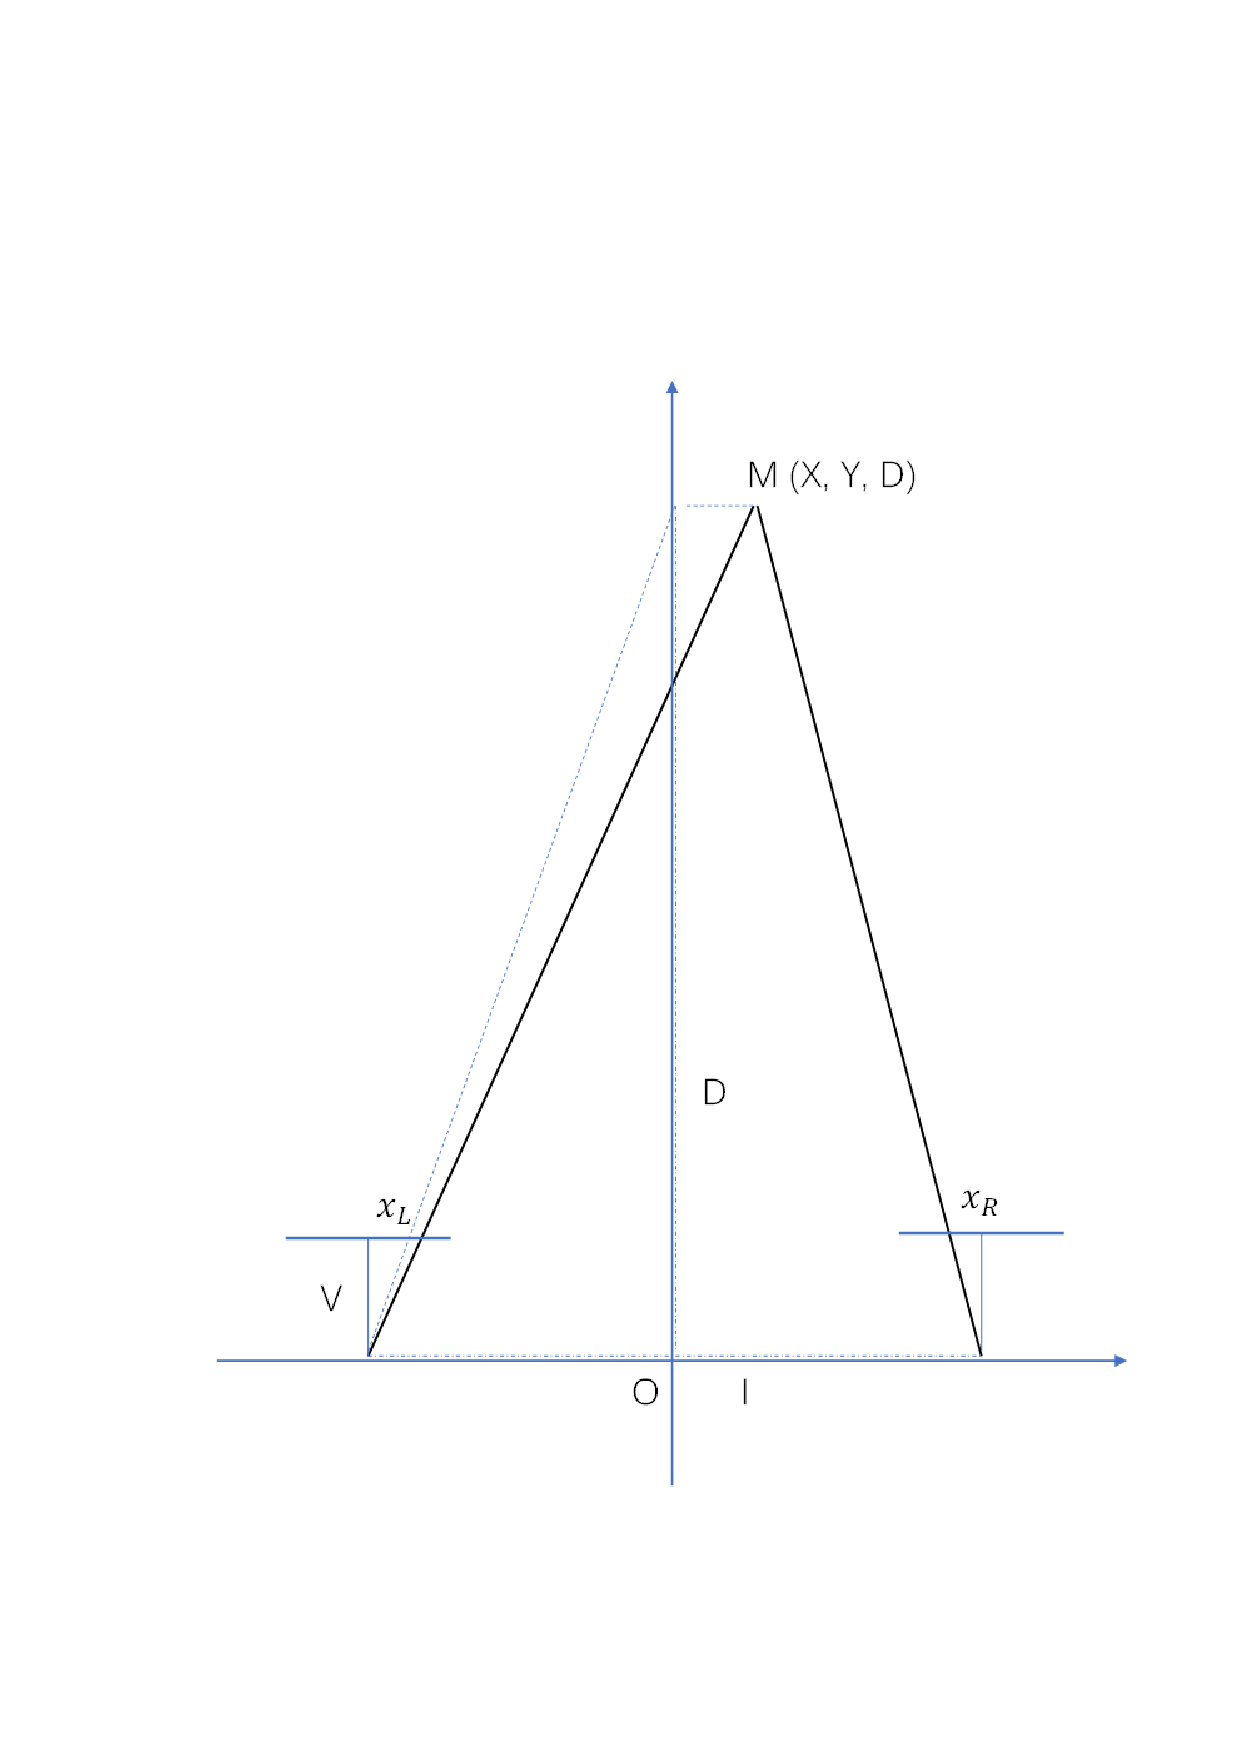
\includegraphics[width=0.5\textwidth]{Drawing1}\\
	\caption{Stereopsis of VR HMD.}
	\label{fig:Stereopsis}
\end{figure}

Our experiments are divided into two parts. In the first part, we investigate the effect of relative depth on luminance adaptation, which is represented by $d_1$. In the second part, the relationship between relative depth and contrast masking effect is investigated and represented by $d_2$.

\subsubsection{Luminance Adaptation}
As is known that the background luminance $bg$ is a factor which affect the visual JND, thus it is also investigated in the VR JND experiments. Based on the aforementioned background information, we design an image pattern to explore the correlation of background luminance $bg$, eccentricity $e$, relative disparity $d$ and JND $T$. The experiment setup is shown as Fig. \ref{fig:Luminance}, and the sketch map of the VR stimuli is shown as Fig. \ref{fig:ContrastSketch}. There is a red cross at the center of the field of view at a constant viewing depth of $D$. During the whole experiment, subjects are requested to fix their attention at this red cross. During each trial, a chessboard noise will appears nearby the red cross in the virtual 3D space. Further more, in order to avoid the influence of predefined location of noise on subjects and help subjects keep their fixation at the center of red cross, the location of the noise is random and depends on three elements: the relative depth $d$ to the red cross in the viewing direction, the retinal eccentricity $e$ between the noise and the fixated red cross, and the central angle of noise to the center. As is known that stereopsis is generated by fusion of similar texture and caused by the dispartiy of the same pixel from different views. However, pure gray background is insufficient to make a three-dimensional experimence for the chessboard noise. To solve this problem, we put a square at center of the field and at the same depth field of the red cross as shown in Fig. \ref{fig:ContrastSketch} to help construct stereopsis. As mentioned, the visual acuity is identical at arbitrary angle of the circle of the same visual eccentricity. Thus JND in the luminance adaptation experiement is determined by the background luminance $bg$, eccentricity $e$ and relative depth $d$.
\begin{figure}[!t]
	\centering
	% Requires \usepackage{graphicx}
	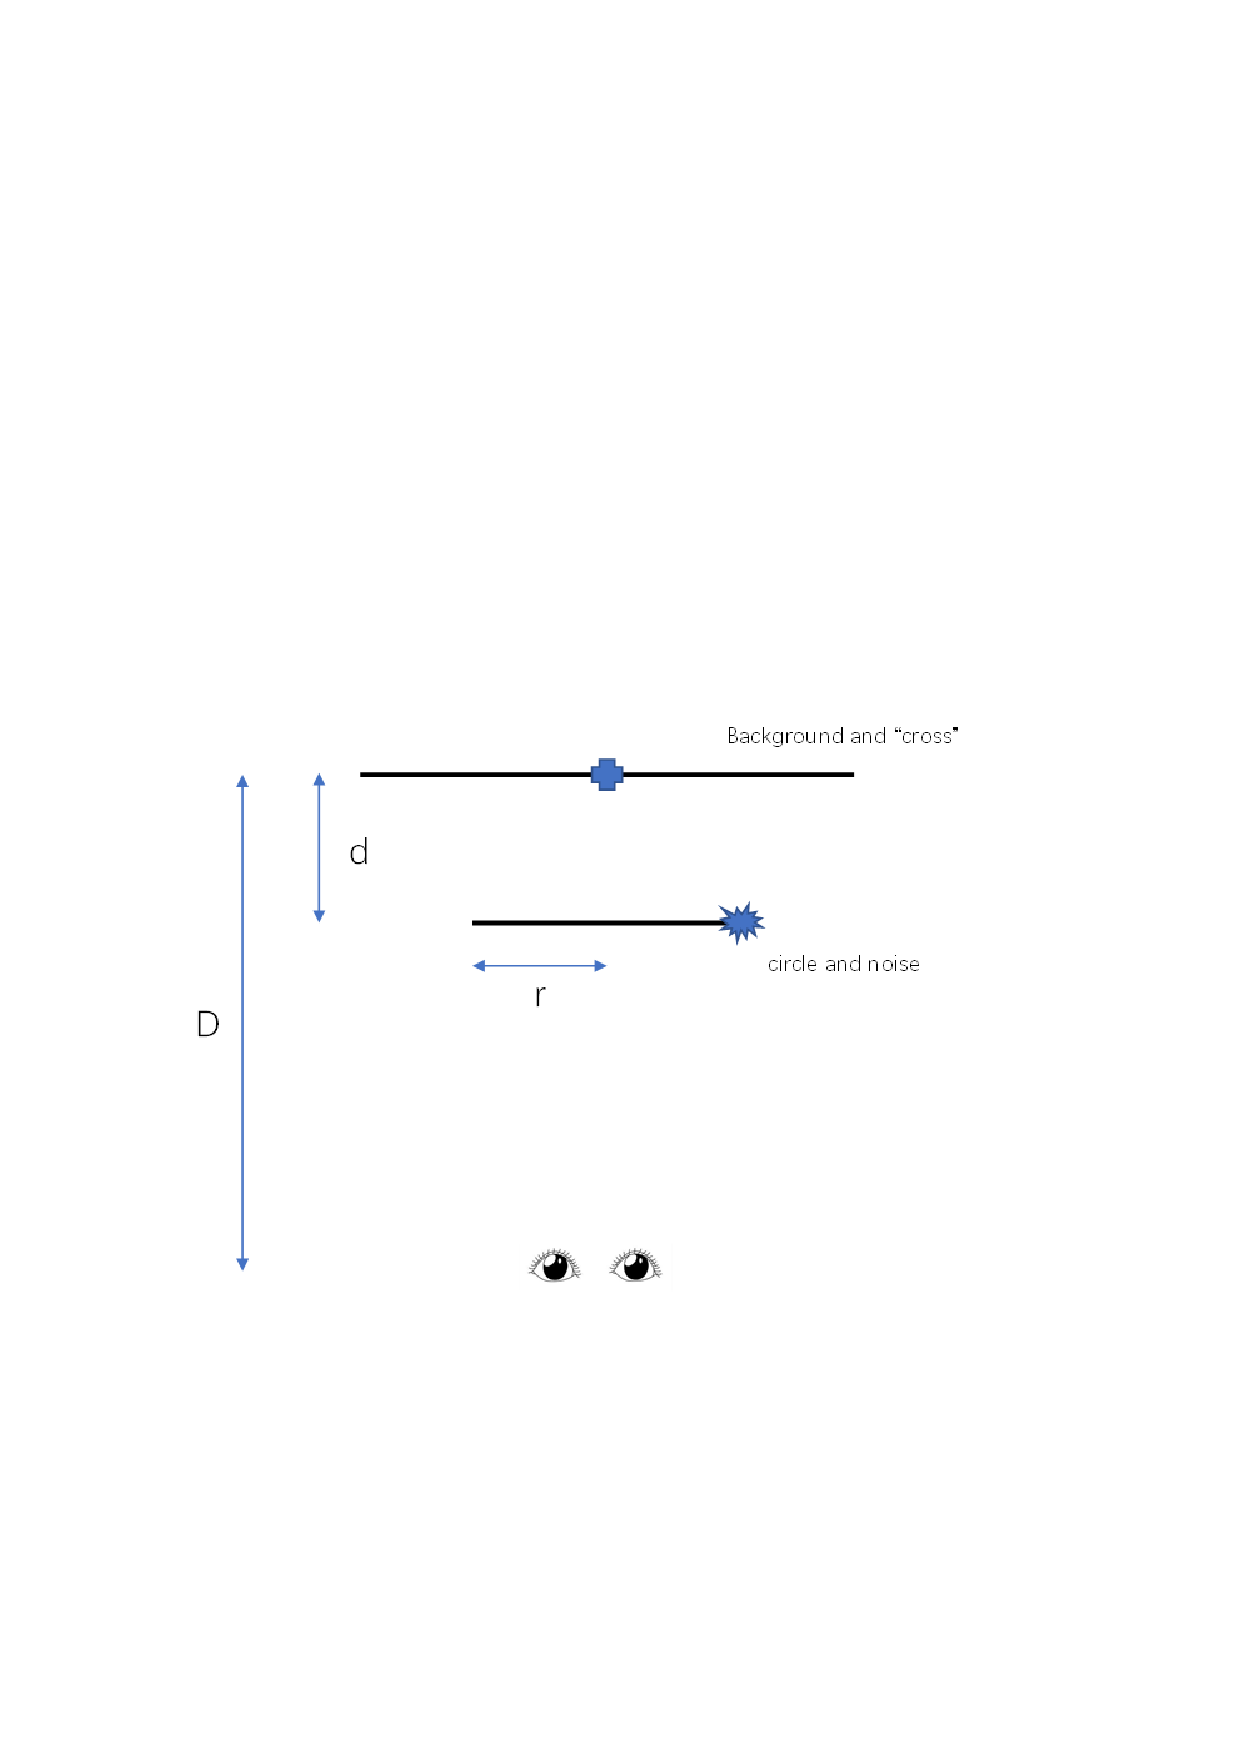
\includegraphics[width=0.5\textwidth]{Drawing2}\\
	\caption{Sketch of luminance adaptation experiment.}
	\label{fig:Luminance}
\end{figure}

\begin{figure}[!t]
	\centering
	% Requires \usepackage{graphicx}
	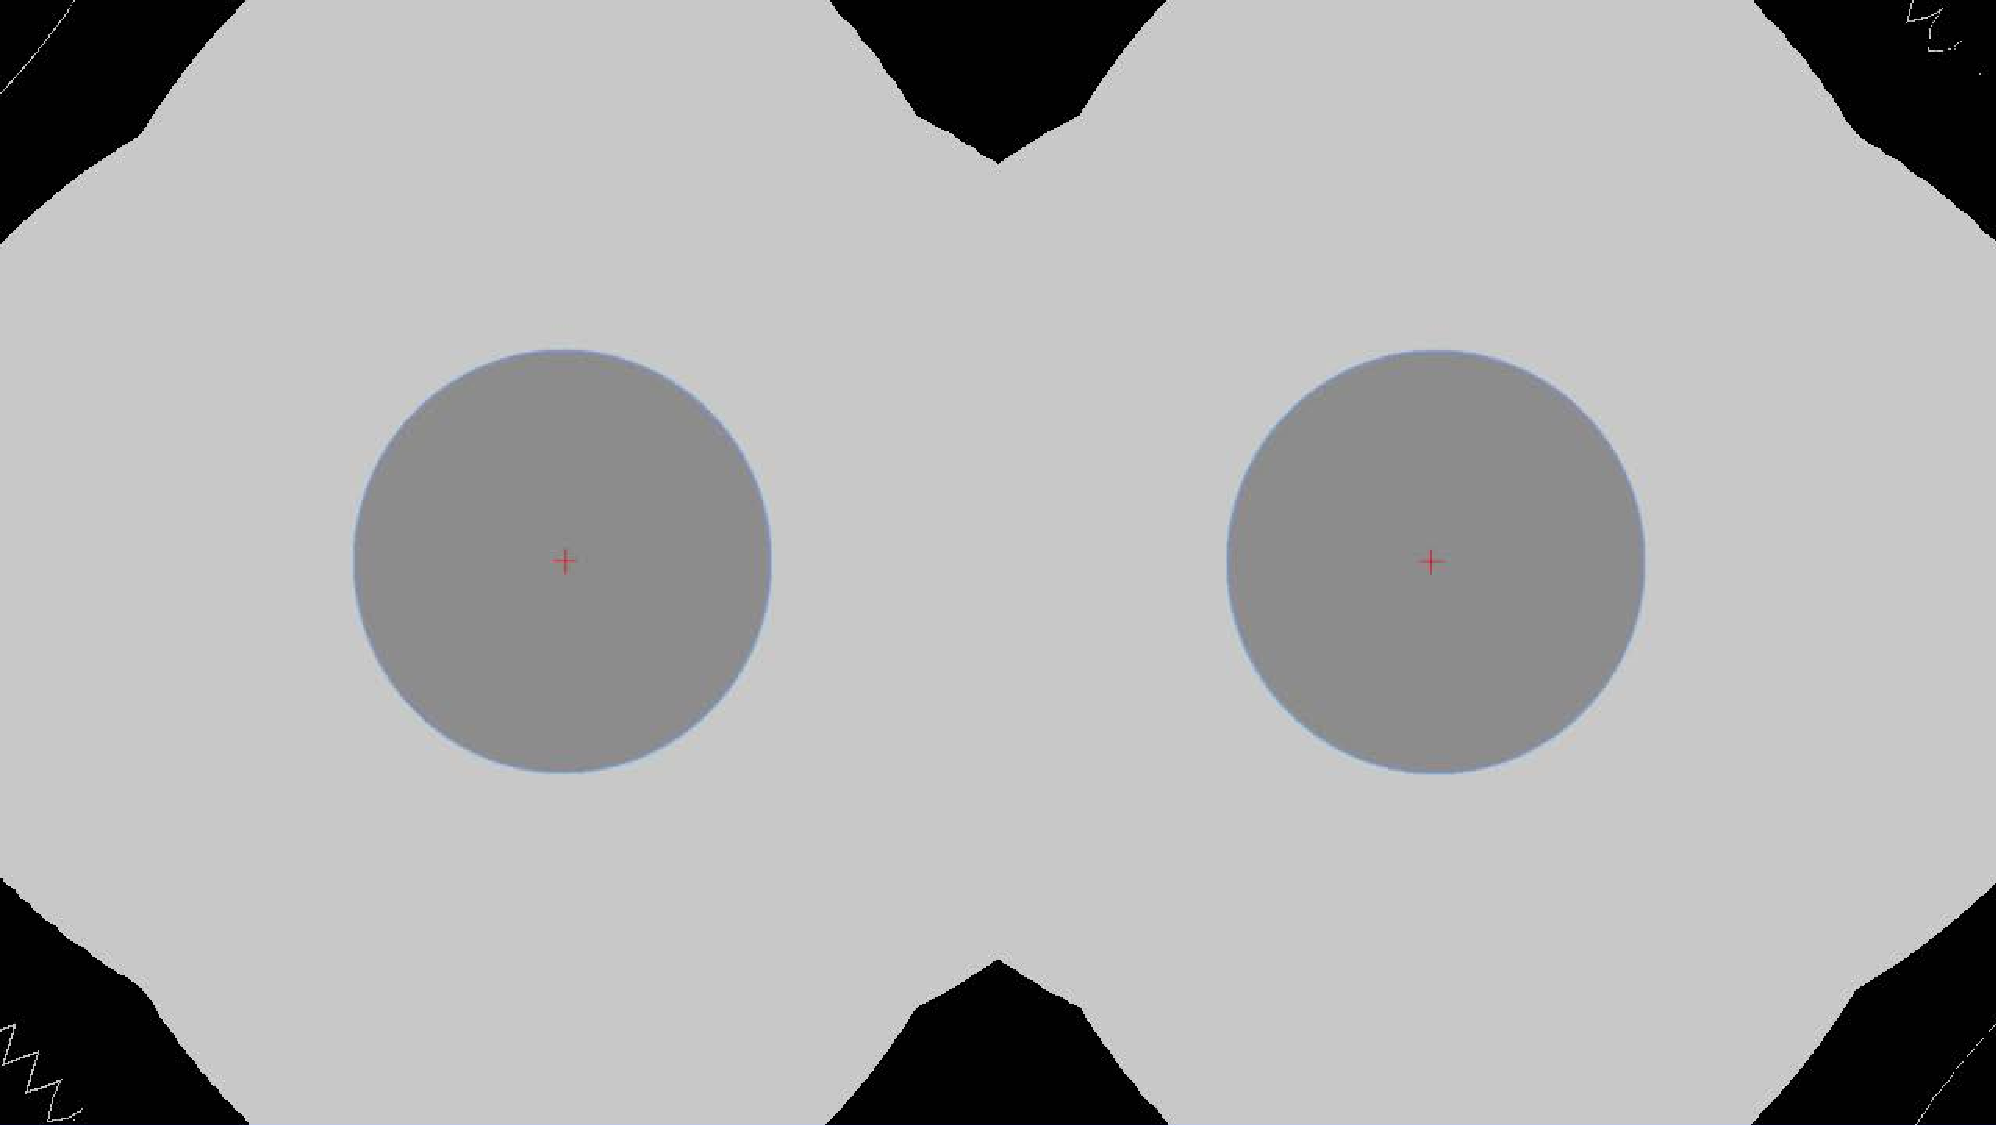
\includegraphics[width=0.48\textwidth]{ContrastSketch}\\
	\caption{Stimuli in the VR glasses of luminance adaptation experiment.}
	\label{fig:ContrastSketch}
	 
\end{figure}
\subsubsection{Contrast Masking}
To investigate the relation The pattern consists of a circular area whose radius is calculated with viewing distance and eccentricity,. 
\section{Experimental Results}

\section{Conclusion}


% Can use something like this to put references on a page
% by themselves when using endfloat and the captionsoff option.
\ifCLASSOPTIONcaptionsoff
  \newpage
\fi

{
	\small
	\bibliographystyle{IEEEtran}
	\bibliography{FD-JND}
}
\end{document}


